\documentclass[11pt,letterpaper]{article}

\usepackage[margin=0.85in]{geometry}
\usepackage[T1]{fontenc}
\usepackage[utf8]{inputenc}
\usepackage{lmodern}
\usepackage{microtype}
\usepackage{graphicx}
\usepackage{booktabs}
\usepackage{array}
\usepackage{xcolor}
\usepackage{hyperref}
\usepackage{caption}
\usepackage{float}
\usepackage{tikz}
\usetikzlibrary{arrows.meta,positioning,shapes.geometric}

\graphicspath{{../../outputs/stage1_td_compare/mix60/}}

\hypersetup{
  colorlinks=true,
  linkcolor=black,
  urlcolor=blue
}

\definecolor{codexblue}{HTML}{1F4E79}
\definecolor{codexorange}{HTML}{C55A11}
\definecolor{softgray}{HTML}{F2F4F7}
\definecolor{warnred}{HTML}{9E2A2B}

\newcommand{\pu}{\mathrm{p.u.}}
\newcommand{\Hz}{\mathrm{Hz}}

\title{\textbf{Stage 1 Dynamic Comparison: IEEE 39 Base Case vs. mix60 IBR Case}}
\author{Spectral IBR validation note}
\date{Generated from ANDES outputs in \texttt{outputs/stage1\_td\_compare/mix60}}

\begin{document}
\maketitle

\begin{abstract}
This note documents the Stage 1 time-domain comparison between the original
IEEE 39 dynamic case and the converted \texttt{mix60} inverter-based resource
(IBR) case. The objective is not to claim that the IBR case is fully validated,
but to check whether ANDES is integrating the intended IBR dynamic models and
whether the response to a common disturbance is physically interpretable. The
final scenario disconnects load \texttt{PQ\_7} at bus 16 at \(t=12\) s. Both
cases run to \(20\) s. The response has the expected sign for a load rejection:
frequency and voltages increase. However, the \texttt{mix60} case shows large
voltage excursions, including buses above \(1.10 \pu\), so the result should be
treated as a successful simulation run with engineering warnings, not as a
final proof of a healthy IBR benchmark.
\end{abstract}

\section{Purpose of the Check}

The question being tested is:

\begin{quote}
Does the converted \texttt{mix60} case actually simulate IBR dynamics in ANDES,
and do the plotted signals make electrical sense for the selected event?
\end{quote}

The answer is conditional. ANDES is using the intended IBR models, and the
qualitative direction of the response is correct. The case is not yet clean
enough to call ``perfect'', because the converted IBR case has stronger voltage
transients than the all-synchronous base case.

\section{What Changed in the Scenario}

The source workbooks are:

\begin{itemize}
  \item Base case: \texttt{data/raw/ieee39\_full.xlsx}.
  \item IBR case: \texttt{data/processed/mix60/mix60.xlsx}.
\end{itemize}

The scenario workbooks generated for this comparison are:

\begin{itemize}
  \item \texttt{outputs/stage1\_td\_compare/mix60/base\_toggle\_pq7.xlsx}.
  \item \texttt{outputs/stage1\_td\_compare/mix60/mix60\_toggle\_pq7.xlsx}.
\end{itemize}

The original workbook includes a disabled \texttt{Toggler} for disconnecting
\texttt{GENROU\_1}. That event was not used for this validation because it is a
large generator outage and caused early termination in the IBR case. A failed
large-contingency run is useful information, but it is not a clean first check
for whether the IBR conversion is wired correctly.

The final scenario keeps the generator toggler disabled and adds one active
load toggler:

\begin{center}
\begin{tabular}{ll}
\toprule
Field & Value \\
\midrule
Model & \texttt{PQ} \\
Device & \texttt{PQ\_7} \\
Bus & 16 \\
Active power & 3.29~p.u. \\
Reactive power & 0.323~p.u. \\
Event time & \(12.0\) s \\
Action & Disconnect load \\
\bottomrule
\end{tabular}
\end{center}

If the system base is 100 MVA, this is approximately a 329 MW and 32.3 MVAr
load rejection. This is not a tiny perturbation; it is a meaningful disturbance.

\section{Experiment Diagram}

\begin{figure}[H]
\centering
\resizebox{\linewidth}{!}{%
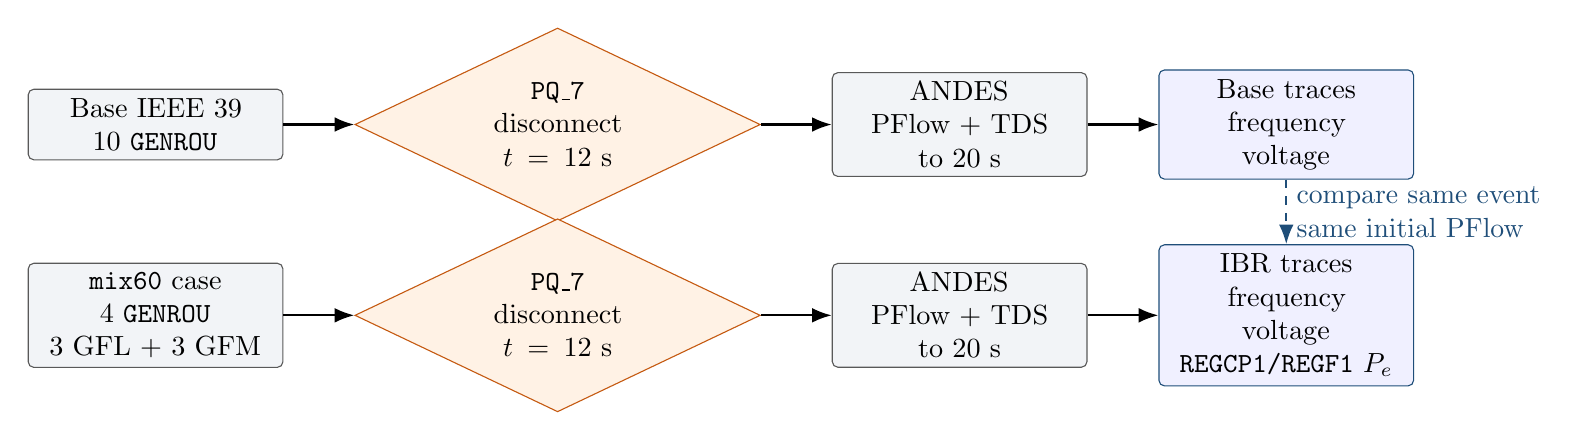
\begin{tikzpicture}[
  node distance=1.0cm and 0.9cm,
  block/.style={
    rectangle,
    rounded corners=2pt,
    draw=black!65,
    fill=softgray,
    align=center,
    minimum height=0.78cm,
    text width=3.0cm
  },
  event/.style={
    diamond,
    aspect=2.1,
    draw=codexorange,
    fill=orange!10,
    align=center,
    inner sep=1.5pt,
    text width=2.6cm
  },
  outputblock/.style={
    rectangle,
    rounded corners=2pt,
    draw=codexblue,
    fill=blue!6,
    align=center,
    minimum height=0.78cm,
    text width=3.0cm
  },
  arrow/.style={-{Latex[length=2.5mm]}, thick}
]

\node[block] (base) {Base IEEE 39\\10 \texttt{GENROU}};
\node[event, right=of base] (event1) {\texttt{PQ\_7}\\disconnect\\\(t=12\) s};
\node[block, right=of event1] (andes1) {ANDES\\PFlow + TDS\\to 20 s};
\node[outputblock, right=of andes1] (plots1) {Base traces\\frequency\\voltage};

\node[block, below=1.3cm of base] (ibr) {\texttt{mix60} case\\4 \texttt{GENROU}\\3 GFL + 3 GFM};
\node[event, right=of ibr] (event2) {\texttt{PQ\_7}\\disconnect\\\(t=12\) s};
\node[block, right=of event2] (andes2) {ANDES\\PFlow + TDS\\to 20 s};
\node[outputblock, right=of andes2] (plots2) {IBR traces\\frequency\\voltage\\\texttt{REGCP1/REGF1} \(P_e\)};

\draw[arrow] (base) -- (event1);
\draw[arrow] (event1) -- (andes1);
\draw[arrow] (andes1) -- (plots1);
\draw[arrow] (ibr) -- (event2);
\draw[arrow] (event2) -- (andes2);
\draw[arrow] (andes2) -- (plots2);

\draw[arrow, dashed, codexblue] (plots1.south) -- node[right, align=left] {
compare same event\\same initial PFlow
} (plots2.north);

\end{tikzpicture}
}
\caption{Stage 1 dynamic comparison workflow. The disturbance is identical in
both workbooks; only the dynamic resource mix changes.}
\end{figure}

\section{IBR Models Actually Present in ANDES}

The \texttt{mix60} case is not only a static spreadsheet change. ANDES loads
dynamic IBR models:

\begin{center}
\begin{tabular}{lcc}
\toprule
Model class & Base case count & \texttt{mix60} count \\
\midrule
\texttt{GENROU} & 10 & 4 \\
\texttt{REGCP1} grid-following IBR & 0 & 3 \\
\texttt{REGF1} grid-forming IBR & 0 & 3 \\
\texttt{REECA1} electrical controller & 0 & 3 \\
\texttt{REPCA1} plant controller & 0 & 3 \\
\texttt{PLL1} phase-locked loop & 0 & 3 \\
\bottomrule
\end{tabular}
\end{center}

The converted generators are:

\begin{itemize}
  \item GFL: generators 5, 7, and 9 at buses 34, 36, and 38.
  \item GFM: generators 4, 6, and 8 at buses 33, 35, and 37.
  \item Synchronous machines retained: buses 30, 31, 32, and 39.
\end{itemize}

\section{Main Numerical Results}

\begin{center}
\begin{tabular}{lcc}
\toprule
Metric & Base case & \texttt{mix60} IBR case \\
\midrule
Final simulation time & 20.0 s & 20.0 s \\
Max frequency delta, selected buses & 0.00131~p.u. & 0.00179~p.u. \\
Approx. max frequency delta & 0.079~Hz & 0.107~Hz \\
Bus 16 max voltage delta & 0.0199~p.u. & 0.0715~p.u. \\
Bus 35 max voltage delta & 0.0150~p.u. & 0.0970~p.u. \\
Max \texttt{REGCP1} \(P_e\) delta & -- & 0.3752~p.u. \\
Max \texttt{REGF1} \(P_e\) delta & -- & 0.6756~p.u. \\
Buses exceeding 1.10~p.u. during TDS & 0 & 20 \\
\bottomrule
\end{tabular}
\end{center}

\section{Interpretation of the Plots}

\subsection{Frequency}

\begin{figure}[H]
\centering
\includegraphics[width=\linewidth]{frequency_busfreq.png}
\caption{Bus frequency response after disconnecting \texttt{PQ\_7}. The
positive frequency change is expected because the event removes load. The
\texttt{mix60} case has a larger final frequency deviation than the base case.}
\end{figure}

The sign of the frequency response is correct. Removing load causes mechanical
input to exceed electrical demand until controls rebalance the system, so
frequency rises. The \texttt{mix60} case rises more than the all-synchronous
base case, which is consistent with lower synchronous inertia and different
active-power control behavior.

\subsection{Voltage}

\begin{figure}[H]
\centering
\includegraphics[width=\linewidth]{voltage_buses.png}
\caption{Voltage response at the disturbance bus and selected generator/IBR
buses. The \texttt{mix60} case has materially larger voltage excursions.}
\end{figure}

The voltage response also has the expected sign. A load rejection reduces local
current and reactive demand, so voltages tend to rise. The concern is the
magnitude. In the \texttt{mix60} run, bus 35 reaches about \(1.157 \pu\), and
20 buses exceed \(1.10 \pu\). This is not a numerical crash, but it is an
engineering warning.

\subsection{IBR Active Power}

\begin{figure}[H]
\centering
\includegraphics[width=\linewidth]{ibr_power.png}
\caption{IBR active power response. Both GFL and GFM devices respond after the
event; oscillations are visible and then damp out.}
\end{figure}

The \texttt{REGCP1} and \texttt{REGF1} traces confirm that the IBR devices are
participating dynamically. The active-power signals move immediately after the
event and then settle. This supports the conclusion that ANDES is integrating
the IBR controls rather than merely preserving a static power-flow injection.

\section{Engineering Concerns}

\begin{enumerate}
  \item The selected event is a load rejection of roughly 329 MW, not a small
  signal test. It is useful, but should not be the only validation scenario.

  \item The \texttt{mix60} voltage response is high. A production validation
  gate should flag or fail cases with voltage maxima above chosen thresholds,
  for example \(1.10 \pu\) warning and \(1.15 \pu\) failure.

  \item Some IBR controller limits are very broad, such as high current and
  reactive-power limits in parts of the GFL control chain. That can make the
  simulation mathematically robust while still being physically optimistic.

  \item The severe original event, disconnecting \texttt{GENROU\_1}, caused
  early termination in prior runs. That result should be documented separately
  as a contingency stress-test failure, not hidden.

  \item A previous attempt to use an \texttt{Alter} load step on \texttt{Ppf}
  and \texttt{Qpf} did not excite the default load model, because default PQ
  loads are converted to impedance/current/power portions for TDS. It is safer
  for this check to use \texttt{Toggler} on a real PQ load device.
\end{enumerate}

\section{Conclusion}

The current Stage 1 comparison demonstrates that:

\begin{itemize}
  \item The base and \texttt{mix60} cases start from the same solved power-flow
  condition.
  \item The \texttt{mix60} case is using dynamic IBR models in ANDES.
  \item The response direction to \texttt{PQ\_7} disconnection is physically
  interpretable: frequency and voltage rise.
  \item The IBR active-power traces move and damp after the event.
\end{itemize}

The result should be reported as:

\begin{quote}
The \texttt{mix60} IBR case simulates successfully in ANDES for the
\texttt{PQ\_7} load-disconnection scenario, and the qualitative response is
consistent with load rejection. However, the voltage excursions are high and
must be treated as engineering warnings. The case is suitable for continued
method development, but not yet as a fully validated benchmark without
additional voltage-limit, controller-limit, and smaller-disturbance tests.
\end{quote}

\end{document}
